\documentclass[journal]{IEEEtran}
\usepackage[a5paper, margin=10mm, onecolumn]{geometry}
\usepackage{tfrupee} 

\setlength{\headheight}{1cm}
\setlength{\headsep}{0mm} 

\usepackage{gvv-book}
\usepackage{gvv}
\usepackage{amsmath,amssymb,amsfonts,amsthm}
\usepackage{algorithmic}
\usepackage{graphicx}
\usepackage{textcomp}
\usepackage{xcolor}
\usepackage{txfonts}
\usepackage{listings}
\usepackage{enumitem}
\usepackage{mathtools}
\usepackage{gensymb}
\usepackage{comment}
\usepackage[breaklinks=true]{hyperref}
\usepackage{tkz-euclide} 
\usepackage{listings}
\def\inputGnumericTable{}                      
\usepackage[latin1]{inputenc}                                
\usepackage{color}                                         
\usepackage{array}                                            
\usepackage{longtable}                                       
\usepackage{calc}                                             
\usepackage{multirow}                                         
\usepackage{hhline}                                           
\usepackage{ifthen}                                           
\usepackage{lscape}
\usepackage{tikz}
\usetikzlibrary{patterns}
\begin{document}


\vspace{3cm}


\title{GATE 2021 - General Aptitude \& Ecology and Evolution (EY)}
\author{ee25btech11034-Kishora Karthik}
\maketitle

{\let\newpage\relax\maketitle}

\renewcommand{\thefigure}{\theenumi}
\renewcommand{\thetable}{\theenumi}
\setlength{\intextsep}{10pt} 

\section*{\textbf{General Aptitude}}
\textbf{Q.1 -- Q.5 Multiple Choice Question (MCQ), carry ONE mark each (for each wrong answer: $-1/3$).}
 
\begin{enumerate}
    \item The people \underline{\hspace{2cm}} who were at the demonstration were from all sections of society.
    \begin{multicols}{2}
    \begin{enumerate}
        \item whose
        \item which
        \item who
        \item whom
    \end{enumerate}
    \end{multicols}
    \hfill{(GATE EY 2021)}

    \item A transparent square sheet shown above is folded along the dotted line. The folded sheet will look like
    \begin{figure}[!h]
        \centering
        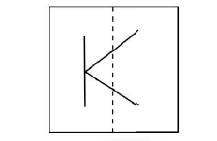
\includegraphics[width=0.4\columnwidth]{figs/Q.2.png}
        \caption{A transparent sheet with the letter K is folded along the dotted line.}
    \end{figure}
    \begin{multicols}{2}
        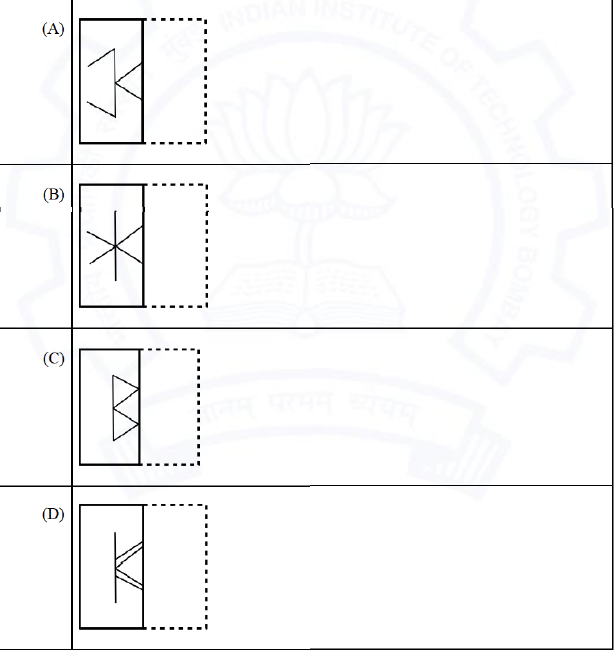
\includegraphics[width=0.5\columnwidth]{figs/Q.2-A.png}
    \end{multicols}
    \hfill{(GATE EY 2021)}

    \item For a regular polygon having $10$ sides, the interior angle between the sides of the polygon, in degrees, is:
    \begin{multicols}{2}
    \begin{enumerate}
        \item $396$
        \item $324$
        \item $216$
        \item $144$
    \end{enumerate}
    \end{multicols}
    \hfill{(GATE EY 2021)}

    \item Which one of the following numbers is exactly divisible by $(11^{13}+1)$?
    \begin{multicols}{2}
    \begin{enumerate}
        \item $11^{26}+1$
        \item $11^{33}+1$
        \item $11^{39}-1$
        \item $11^{52}-1$
    \end{enumerate}
    \end{multicols}
    \hfill{(GATE EY 2021)}

    \item Oasis is to sand as island is to \underline{\hspace{3cm}}. \\
    Which one of the following options maintains a similar logical relation in the above sentence?
    \begin{multicols}{2}
    \begin{enumerate}
        \item Stone
        \item Land
        \item Water
        \item Mountain
    \end{enumerate}
    \end{multicols}
    \hfill{(GATE EY 2021)}

\textbf{Q.6 -- Q.10 Multiple Choice Question (MCQ), carry TWO marks each (for each wrong answer: $-2/3$).}
 
    \item The importance of sleep is often overlooked by students when they are preparing for exams. Research has consistently shown that sleep deprivation greatly reduces the ability to recall the material learnt. Hence, cutting down on sleep to study longer hours can be counterproductive. \\
    Which one of the following statements is the CORRECT inference from the above passage?
    \begin{enumerate}
        \item Sleeping well alone is enough to prepare for an exam. Studying has lesser benefit.
        \item Students are efficient and are not wrong in thinking that sleep is a waste of time.
        \item If a student is extremely well prepared for an exam, he needs little or no sleep.
        \item To do well in an exam, adequate sleep must be part of the preparation.
    \end{enumerate}
    \hfill{(GATE EY 2021)}

    \item In the figure shown above, each inside square is formed by joining the midpoints of the sides of the next larger square. The area of the smallest square (shaded) as shown, in $cm^{2}$ is:
    \begin{figure}[!h]
        \centering
        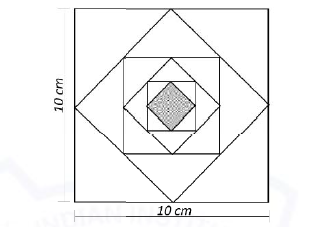
\includegraphics[width=0.2\columnwidth]{figs/Q.7.png}
        \caption{Nested squares formed by joining midpoints. Outermost square is $10$ cm x $10$ cm.}
        \label{Q.7}
    \end{figure}
    \begin{multicols}{2}
    \begin{enumerate}
        \item $12.50$
        \item $6.25$
        \item $3.125$
        \item $1.5625$
    \end{enumerate}
    \end{multicols}
    \hfill{(GATE EY 2021)}

    \item Let $X$ be a continuous random variable denoting the temperature measured. The range of temperature is $[0, 100]$ degree Celsius and let the probability density function of $X$ be $f(x)=0.01$ for $0 \le X \le 100$. The mean of $X$ is
    \begin{multicols}{2}
    \begin{enumerate}
        \item $2.5$
        \item $5.0$
        \item $25.0$
        \item $50.0$
    \end{enumerate}
    \end{multicols}
    \hfill{(GATE EY 2021)}

    \item The number of students passing or failing in an exam for a particular subject are presented in the bar chart above. Students who pass the exam cannot appear for the exam again. Students who fail the exam in the first attempt must appear for the exam in the following year. Students always pass the exam in their second attempt.
    \begin{figure}[!h]
        \centering
        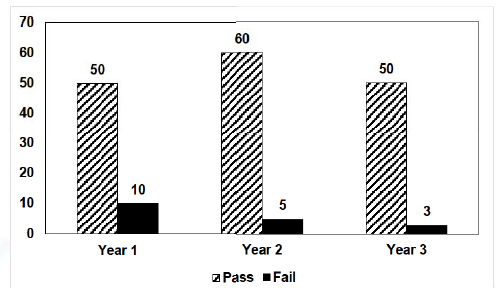
\includegraphics[width=0.3\columnwidth]{figs/Q.9.png}
        \caption{Bar chart showing Pass/Fail count for Year 1, 2, and 3.}
    \end{figure}
    The number of students who took the exam for the first time in the year 2 and the year 3 respectively, are
    \begin{multicols}{2}
    \begin{enumerate}
        \item $65$ and $53$
        \item $60$ and $50$
        \item $55$ and $53$
        \item $55$ and $48$
    \end{enumerate}
    \end{multicols}
    \hfill{(GATE EY 2021)}

    \item Seven cars P, Q, R, S, T, U and V are parked in a row not necessarily in that order. The cars T and U should be parked next to each other. The cars S and V also should be parked next to each other, whereas P and Q cannot be parked next to each other. Q and S must be parked next to each other. R is parked to the immediate right of V. T is parked to the left of U. \\
    Based on the above statements, the only INCORRECT option given below is:
    \begin{enumerate}
        \item There are two cars parked in between Q and V.
        \item Q and R are not parked together.
        \item V is the only car parked in between S and R.
        \item Car P is parked at the extreme end.
    \end{enumerate}
    \hfill{(GATE EY 2021)}

\end{enumerate}
\clearpage

\section*{\textbf{Ecology and Evolution (EY)}}
\textbf{Q.1 -- Q.16 Multiple Choice Question (MCQ), carry ONE mark each (for each wrong answer: $-1/3$).}
\begin{enumerate}

    \item Animal species can vary in whether dispersal is more likely among male offspring (male-biased), female offspring (female-biased), or similar between the sexes. Dispersal in birds and mammals is most commonly
    \begin{enumerate}
        \item female-biased and male-biased, respectively.
        \item female-biased and similar between the sexes, respectively.
        \item male-biased and female-biased, respectively.
        \item similar between the sexes, and female-biased respectively.
    \end{enumerate}
    \hfill{(GATE EY 2021)}

    \item Of the following, which one is the most direct measure of Darwinian fitness?
    \begin{multicols}{2}
    \begin{enumerate}
        \item Adult body size
        \item Lifetime reproductive success
        \item Lifespan
        \item Maximum sprint speed
    \end{enumerate}
    \end{multicols}
    \hfill{(GATE EY 2021)}

    \item The marginal value theorem in optimal foraging theory examines which one of the following foraging decisions?
    \begin{enumerate}
        \item How long to stay in a patch of food
        \item How to allocate time to foraging versus reproduction
        \item How to minimise risk while foraging
        \item How to select between different food types within a patch
    \end{enumerate}
    \hfill{(GATE EY 2021)}

    \item Which one of the following shows the highest degree of endemism?
    \begin{multicols}{2}
    \begin{enumerate}
        \item Birds of the Himalayas
        \item Mammals of central India
        \item Frogs of the Western Ghats
        \item Trees of the Gangetic basin
    \end{enumerate}
    \end{multicols}
    \hfill{(GATE EY 2021)}
    
    \item Which one of the following Mendelian disorders is influenced by diet?
    \begin{multicols}{2}
    \begin{enumerate}
        \item Cystic fibrosis
        \item Haemophilia
        \item Phenylketonuria
        \item Thalassemia
    \end{enumerate}
    \end{multicols}
    \hfill{(GATE EY 2021)}

    \item Which one of the following mammalian DNA regions exhibits the highest level of sequence variation?
    \begin{enumerate}
        \item Homeobox transcription factor binding domain
        \item Hox genes
        \item Mitochondrial D-loop region
        \item Histone protein-encoding genes
    \end{enumerate}
    \hfill{(GATE EY 2021)}

    \item Which one of the following makes a species most vulnerable to extinction?
    \begin{enumerate}
        \item Low density throughout a large geographic range and in several habitat types
        \item Locally common in a restricted geographic range and in several habitat types
        \item Low density throughout a large geographic range and in a specific habitat type
        \item Locally common in a restricted geographic range and in a specific habitat type
    \end{enumerate}
    \hfill{(GATE EY 2021)}

    \item The frequency distributions of a trait in two populations, $X$ and $Y$, are shown in the figure. Which one of the following statements about the mean and standard deviation ($SD$) of the two populations is accurate?
    \begin{figure}[!h]
        \centering
        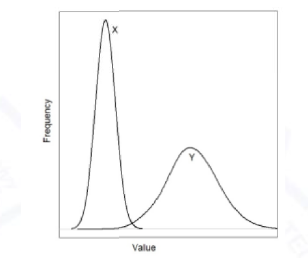
\includegraphics[width=0.3\columnwidth]{figs/Q.8.png}
        \caption{Frequency distributions for populations X and Y.}
        \label{Q.8}
    \end{figure}
    \begin{enumerate}
        \item $X$ has higher mean, and $Y$ has higher $SD$.
        \item $Y$ has higher mean, and $X$ has higher $SD$.
        \item $X$ has higher mean, and $X$ has higher $SD$.
        \item $Y$ has higher mean, and $Y$ has higher $SD$.
    \end{enumerate}
    \hfill{(GATE EY 2021)}

    \item Two sister species of bulbuls have non-overlapping distributions. One is distributed in India and the other in Sri Lanka. Which one of the following modes of speciation is the most parsimonious explanation for this pattern?
    \begin{multicols}{2}
    \begin{enumerate}
        \item Allopatric speciation
        \item Sympatric speciation
        \item Parapatric speciation
        \item Peripatric speciation
    \end{enumerate}
    \end{multicols}
    \hfill{(GATE EY 2021)}

    \item In an Arctic Ocean food chain, killer whales feed on sea otters, which feed on sea urchins, which in turn feed on kelp (a type of seaweed). An increase in the abundance of killer whales causes sea otter abundance to decline, leading to higher sea urchin densities, which in turn reduces the abundance of kelp. Which one of the following terms describes this phenomenon?
    \begin{multicols}{2}
    \begin{enumerate}
        \item Trophic cascade
        \item Prey switching
        \item Competitive exclusion
        \item Productivity-stability relationship
    \end{enumerate}
    \end{multicols}
    \hfill{(GATE EY 2021)}

    \item Listed below are hypotheses for the evolution of monogamy. Which one of these is NOT based on the concept of individual selection?
    \begin{enumerate}
        \item Food provisioning by both parents is crucial for offspring survival.
        \item Biparental protection from predators is essential for offspring survival.
        \item Females are solitary and dispersed; therefore, males cannot effectively mate-guard more than one female at a time.
        \item Forming monogamous pairs allows individuals to regulate their reproductive output and ensure the survival of the species.
    \end{enumerate}
    \hfill{(GATE EY 2021)}

    \item Rising temperature due to global warming can stimulate decomposition of organic matter and release $CO_2$ into the atmosphere. This is an example of
    \begin{multicols}{2}
    \begin{enumerate}
        \item positive feedback.
        \item negative feedback.
        \item environmental heterogeneity.
        \item environmental stochasticity.
    \end{enumerate}
    \end{multicols}
    \hfill{(GATE EY 2021)}

    \item Ant-mimic spiders of the genus \textit{Myrmarachne} are known for which one of the following evolutionary phenomena?
    \begin{multicols}{2}
    \begin{enumerate}
        \item Aposematism
        \item Aggressive mimicry
        \item Batesian mimicry
        \item Muellerian mimicry
    \end{enumerate}
    \end{multicols}
    \hfill{(GATE EY 2021)}

    \item The probability of local extinction of a species increases with body size when there is forest degradation, loss, and fragmentation. Consider the following hypotheses for the vulnerability of larger-bodied species: \\
    (P) Larger-bodied species tend to have smaller population sizes. \\
    (Q) Larger-bodied species require larger territories/home ranges. \\
    (R) Larger-bodied species have higher absolute resource and energy requirements. \\
    Which one of the following options correctly lists all potential reasons for the vulnerability of larger-bodied species?
    \begin{multicols}{2}
    \begin{enumerate}
        \item P and Q only
        \item P only
        \item P and R only
        \item P, Q, and R
    \end{enumerate}
    \end{multicols}
    \hfill{(GATE EY 2021)}

    \item Grazing by large mammalian herbivores can have a strong influence on ecosystem structure, and can cause ecosystems to transition between alternative states over decades. Which one of the following transitions can result from grazing?
    \begin{multicols}{2}
    \begin{enumerate}
        \item Mangrove to coral reef
        \item Terai grassland to alpine meadow
        \item Savanna to grassland
        \item Tropical rainforest to arid desert
    \end{enumerate}
    \end{multicols}
    \hfill{(GATE EY 2021)}

    \item The effective population size of a sexually reproducing, diploid, animal species will be highest when the sex ratio (number of reproducing males / number of reproducing females) is
    \begin{multicols}{4}
    \begin{enumerate}
        \item $1$
        \item $0.5$
        \item $1.5$
        \item $2$
    \end{enumerate}
    \end{multicols}
    \hfill{(GATE EY 2021)}

\textbf{Q.17 -- Q.25 Numerical Answer Type (NAT), carry ONE mark each (no negative marks).}

    \item According to Hamilton's rule, a costly altruistic act is favoured by kin selection if $c < rb$, where $c$ is the cost to the actor, $b$ is the benefit to the recipient, and $r$ is the coefficient of relatedness between the actor and the recipient. If a monarch butterfly lays an egg on a plant, there is a cost of $3$ units to its own future reproduction. The egg has a $50\%$ chance of producing a female, that will have $10$ offspring. If the monarch instead decides to not lay an egg and helps its sister, which has a clutch of $8$ eggs, all of which survive and reproduce, the number of its own offspring equivalents it has gained is \underline{\hspace{3cm}}. (Round off to one decimal place)
    \hfill{(GATE EY 2021)}

    \item A single locus with two alleles, A and a, determines coat colour in a rodent. The frequency of the dominant phenotype in a population is $0.96$. Assuming that this locus is in Hardy-Weinberg equilibrium, the frequency of the heterozygous genotype is \underline{\hspace{3cm}}. (Round off to two decimal places)
    \hfill{(GATE EY 2021)}

    \item A researcher is studying the relationship between the height ($y$, in cm) and seed diameter ($x$, in mm) of a plant. The following linear model describes this relationship: $y = 0.5x - 1.2$. The predicted height of a plant that has a seed diameter of $10$ mm is \underline{\hspace{3cm}} cm.
    \hfill{(GATE EY 2021)}

    \item An area of $100$ hectares has a total of $5000$ individuals of a tree species. The population density of this species is \underline{\hspace{3cm}} individuals per hectare.
    \hfill{(GATE EY 2021)}

    \item The frequency of an allele 'a' in a population is $0.4$. If the population is in Hardy-Weinberg equilibrium, the percentage of heterozygous individuals in this population is \underline{\hspace{3cm}}.
    \hfill{(GATE EY 2021)}

    \item To estimate the number of snakes in a population, a researcher captures, marks, and releases $40$ snakes. A week later, she captures $50$ snakes and finds that $10$ of them are marked. The estimated number of snakes in this population is \underline{\hspace{3cm}}.
    \hfill{(GATE EY 2021)}

    \item In a population that follows the logistic growth model, the carrying capacity is $K=500$ and the intrinsic rate of increase is $r=0.2$. The maximum rate of population growth ($dN/dt$) is \underline{\hspace{3cm}}.
    \hfill{(GATE EY 2021)}

    \item The body length ($S$, in mm) of an insect was measured on a set of $100$ individuals. The mean body length was $20$ mm. The heritability of body length was estimated to be $0.4$. A group of individuals with a mean body length of $25$ mm was used to breed the next generation. The expected response to selection ($R$, in mm) is \underline{\hspace{3cm}}.
    \hfill{(GATE EY 2021)}

    \item In a particular ecosystem, the species-area relationship is given by the equation $S = 2.5 A^{0.5}$, where S is the number of species and A is the area of the ecosystem in hectares. The number of species in an area of $100$ hectares is \underline{\hspace{3cm}}.
    \hfill{(GATE EY 2021)}

\textbf{Q.26 -- Q.45 Multiple Choice Question (MCQ), carry TWO marks each (for each wrong answer: $-2/3$).}

    \item The relative abundance of C3 plants is expected to be higher than C4 plants
    \begin{enumerate}
        \item at high temperatures, high solar radiation, and low $CO_2$.
        \item at low temperatures, low solar radiation, and high $CO_2$.
        \item at low temperatures, high solar radiation, and low $CO_2$.
        \item at high temperatures, low solar radiation, and high $CO_2$.
    \end{enumerate}
    \hfill{(GATE EY 2021)}

    \item Semelparous organisms are those that produce all of their offspring in a single reproductive event. Which of the following life-history trade-offs is most likely to favour the evolution of semelparity?
    \begin{enumerate}
        \item A positive trade-off between fecundity and survival.
        \item A negative trade-off between offspring size and offspring number.
        \item A negative trade-off between current and future reproduction.
        \item A positive trade-off between offspring size and survival.
    \end{enumerate}
    \hfill{(GATE EY 2021)}

    \item Bird species X and Y have similar diets and are found in the same habitats. Species X has a long, thin beak and is a specialist forager. Species Y has a short, thick beak and is a generalist forager. Which of the following statements is a plausible hypothesis for the co-occurrence of these two species?
    \begin{enumerate}
        \item X is a better competitor than Y.
        \item Y is a better competitor than X.
        \item X and Y are limited by different resources.
        \item X and Y have similar competitive abilities.
    \end{enumerate}
    \hfill{(GATE EY 2021)}
    
    \item A researcher is interested in the effect of island size on the diversity of species. She surveys a series of islands of different sizes and finds that larger islands have more species. Which of the following is NOT a plausible explanation for this pattern?
    \begin{enumerate}
        \item Larger islands have higher rates of immigration.
        \item Larger islands have lower rates of extinction.
        \item Larger islands have more habitat diversity.
        \item Larger islands have higher rates of speciation.
    \end{enumerate}
    \hfill{(GATE EY 2021)}

    \item The theory of parent-offspring conflict predicts that
    \begin{enumerate}
        \item parents and offspring will always agree on the amount of parental investment.
        \item parents will always invest more in their offspring than the offspring desire.
        \item offspring will always want more parental investment than the parents are willing to provide.
        \item parents and offspring will disagree on the timing of reproduction.
    \end{enumerate}
    \hfill{(GATE EY 2021)}

    \item A species of fish has a diet that consists of both zooplankton and algae. In the presence of a predator, the fish reduces its foraging activity on zooplankton and increases its foraging activity on algae. This is an example of
    \begin{enumerate}
        \item an indirect effect of the predator on the algae.
        \item a direct effect of the predator on the algae.
        \item a trophic cascade.
        \item competitive exclusion.
    \end{enumerate}
    \hfill{(GATE EY 2021)}

    \item Genetic drift is a process that
    \begin{enumerate}
        \item increases genetic variation within a population.
        \item decreases genetic variation within a population.
        \item increases genetic variation between populations.
        \item decreases genetic variation between populations.
    \end{enumerate}
    \hfill{(GATE EY 2021)}
    
    \item The figure below shows the population dynamics of a predator and its prey, according to the Lotka-Volterra model. Which of the panels (i, ii, iii, iv) represents the prey population dynamics in the absence of the predator?
    \begin{figure}[!h]
        \centering
        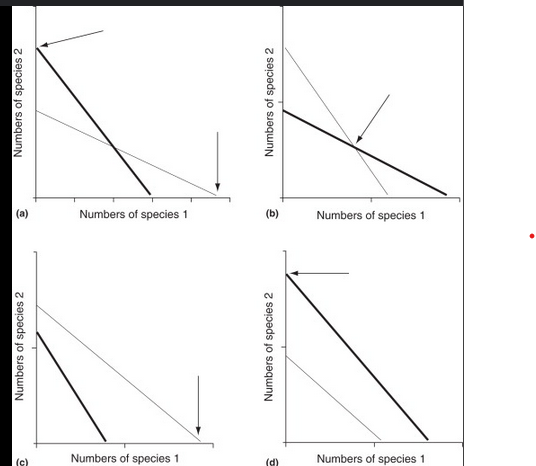
\includegraphics[width=0.6\columnwidth]{figs/Q.33.png}
        \caption{Lotka-Volterra predator-prey dynamics.}
        \label{Q.33}
    \end{figure}
    \begin{multicols}{4}
    \begin{enumerate}
        \item (i)
        \item (ii)
        \item (iii)
        \item (iv)
    \end{enumerate}
    \end{multicols}
    \hfill{(GATE EY 2021)}

    \item Which of the following is NOT a plausible explanation for the evolution of altruism?
    \begin{multicols}{2}
    \begin{enumerate}
        \item Kin selection
        \item Group selection
        \item Reciprocal altruism
        \item Individual selection
    \end{enumerate}
    \end{multicols}
    \hfill{(GATE EY 2021)}

    \item The phylogenetic tree below shows the evolutionary relationships between five species (A, B, C, D, and E). Which of the following statements is correct?
    \begin{figure}[!h]
        \centering
        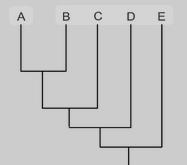
\includegraphics[width=0.5\columnwidth]{figs/Q.35.png}
        \label{Q.35}
        \caption{Phylogenetic tree of five species.}
    \end{figure}
    \begin{enumerate}
        \item A is more closely related to B than to C.
        \item C is more closely related to D than to E.
        \item A and B are sister taxa.
        \item E is the outgroup.
    \end{enumerate}
    \hfill{(GATE EY 2021)}

    \item A species of bird disperses the seeds of a particular tree. Which of the following is LEAST likely to be an adaptation of the bird for this interaction?
    \begin{enumerate}
        \item A gizzard that grinds seeds.
        \item A preference for the fruit of the tree.
        \item A digestive system that does not damage the seeds.
        \item A ranging behaviour that results in the deposition of seeds in suitable habitats.
    \end{enumerate}
    \hfill{(GATE EY 2021)}

    \item The Resource Availability Hypothesis predicts that
    \begin{enumerate}
        \item plants in resource-rich environments will invest more in defence.
        \item plants in resource-poor environments will invest more in defence.
        \item plants will invest in defence only when they are attacked by herbivores.
        \item plants will not invest in defence if they have other means of protection.
    \end{enumerate}
    \hfill{(GATE EY 2021)}

    \item In a species of bird, males with brighter plumage have higher mating success. However, males with brighter plumage are also more conspicuous to predators. This is an example of
    \begin{enumerate}
        \item sexual selection balancing natural selection.
        \item sexual selection reinforcing natural selection.
        \item genetic drift.
        \item gene flow.
    \end{enumerate}
    \hfill{(GATE EY 2021)}

    \item Which of the following is a key assumption of the metapopulation model proposed by Levins?
    \begin{enumerate}
        \item All patches are of equal size and quality.
        \item The rate of colonization is independent of the number of occupied patches.
        \item The rate of extinction is independent of the number of occupied patches.
        \item The metapopulation is always at equilibrium.
    \end{enumerate}
    \hfill{(GATE EY 2021)}

    \item Which of the following is NOT a plant secondary metabolite?
    \begin{multicols}{2}
    \begin{enumerate}
        \item Alkaloids
        \item Terpenoids
        \item Cellulose
        \item Phenolics
    \end{enumerate}
    \end{multicols}
    \hfill{(GATE EY 2021)}

    \item The 'handicap principle' is an explanation for
    \begin{enumerate}
        \item the evolution of honest signals.
        \item the evolution of deceptive signals.
        \item the evolution of altruism.
        \item the evolution of cooperation.
    \end{enumerate}
    \hfill{(GATE EY 2021)}
    
    \item The age structure of a population is shown in the figure below. Which of the following statements is the most likely description of this population?
    \begin{figure}[!h]
        \centering
        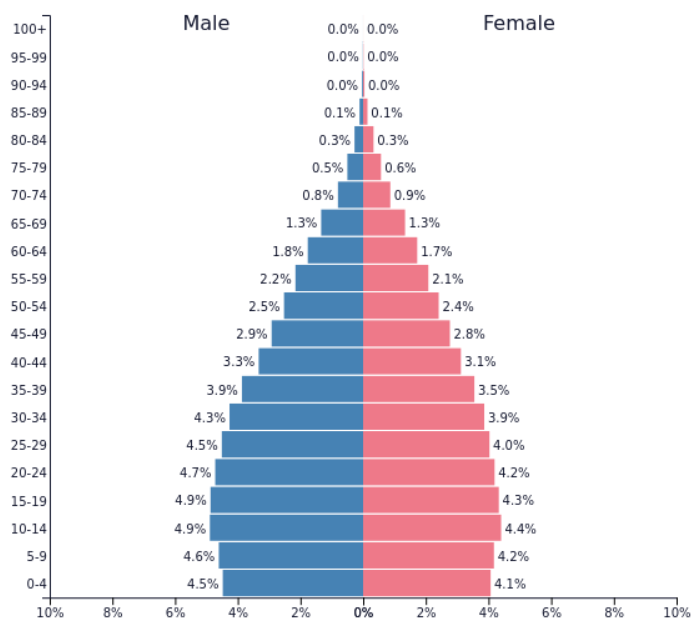
\includegraphics[width=0.4\columnwidth]{figs/Q.42.png}
        \label{Q.42}
        \caption{Population age pyramid.}
    \end{figure}
    \begin{enumerate}
        \item It is a rapidly growing population.
        \item It is a stable population.
        \item It is a declining population.
        \item It is a population with a high death rate.
    \end{enumerate}
    \hfill{(GATE EY 2021)}
    
    \item The coefficient of relatedness between an individual and its full cousin (the offspring of its parent's full sibling) is
    \begin{multicols}{2}
    \begin{enumerate}
        \item $0.5$
        \item $0.25$
        \item $0.125$
        \item $0.0625$
    \end{enumerate}
    \end{multicols}
    \hfill{(GATE EY 2021)}

    \item A researcher sequenced a gene from four species (A, B, C, and D) and obtained the following alignment. Assuming that the most parsimonious tree is the true tree, which of the following trees represents the correct evolutionary relationships between the species?
    \begin{verbatim}
    Species A: A T T G C C
    Species B: A T C G C C
    Species C: A T C G T C
    Species D: A T T G T C
    \end{verbatim}
    \begin{figure}[!h]
        \centering
        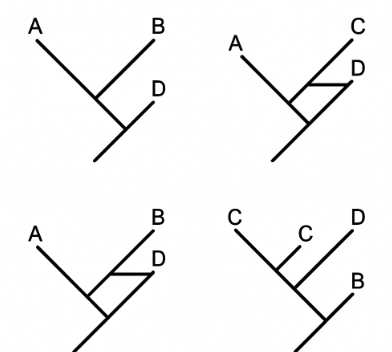
\includegraphics[width=0.7\columnwidth]{figs/Q.44.png}
        \label{Q.44}
        \caption{Four possible phylogenetic trees.}
    \end{figure}
    \begin{multicols}{4}
    \begin{enumerate}
        \item Tree 1
        \item Tree 2
        \item Tree 3
        \item Tree 4
    \end{enumerate}
    \end{multicols}
    \hfill{(GATE EY 2021)}

    \item Eusociality is a form of social behaviour characterized by cooperative brood care, overlapping generations, and a division of labour into reproductive and non-reproductive castes. Which of the following is NOT a eusocial insect?
    \begin{multicols}{4}
    \begin{enumerate}
        \item Honeybees
        \item Termites
        \item Ants
        \item Butterflies
    \end{enumerate}
    \end{multicols}
    \hfill{(GATE EY 2021)}

\textbf{Q.46 -- Q.55 Multiple Select Question (MSQ), carry TWO marks each. A question may have one or more correct answers.}

    \item Which of the following factors can influence the species diversity of a community?
    \begin{enumerate}
        \item The size of the community.
        \item The age of the community.
        \item The level of disturbance in the community.
        \item The productivity of the community.
    \end{enumerate}
    \hfill{(GATE EY 2021)}
    
    \item Which of the following statements about ecological succession is/are correct?
    \begin{enumerate}
        \item Succession is a directional change in the species composition of a community over time.
        \item Primary succession occurs on newly formed habitats, while secondary succession occurs on disturbed habitats.
        \item The climax community is the final stage of succession and is stable over time.
        \item The rate of succession is always slow.
    \end{enumerate}
    \hfill{(GATE EY 2021)}

    \item Coevolution can occur between which of the following pairs of interacting species?
    \begin{enumerate}
        \item Predator and prey
        \item Host and parasite
        \item Plant and pollinator
        \item Competitors
    \end{enumerate}
    \hfill{(GATE EY 2021)}
    
    \item Which of the following are plant hormones?
    \begin{multicols}{4}
    \begin{enumerate}
        \item Auxin
        \item Gibberellin
        \item Cytokinin
        \item Ethylene
    \end{enumerate}
    \end{multicols}
    \hfill{(GATE EY 2021)}
    
    \item Which of the following can regulate population size?
    \begin{enumerate}
        \item Density-dependent factors
        \item Density-independent factors
        \item Intraspecific competition
        \item Interspecific competition
    \end{enumerate}
    \hfill{(GATE EY 2021)}
    
    \item Which of the following is/are key innovations in the evolution of vertebrates?
    \begin{multicols}{4}    
    \begin{enumerate}
        \item Jaws
        \item Lungs
        \item Amniotic egg
        \item Feathers
    \end{enumerate}
    \end{multicols}
    \hfill{(GATE EY 2021)}
    
    \item Which of the following are considered ecosystem services?
     \begin{multicols}{2}
    \begin{enumerate}   
        \item Pollination
        \item Pest control
        \item Water purification
        \item Climate regulation
    \end{enumerate}
    \end{multicols}
    \hfill{(GATE EY 2021)}
    
    \item Which of the following enzymes is/are involved in DNA replication?
     \begin{multicols}{4}
    \begin{enumerate}
        \item DNA polymerase
        \item DNA ligase
        \item Helicase
        \item Primase
    \end{enumerate}
    \end{multicols}
    \hfill{(GATE EY 2021)}
    
    \item Biodiversity hotspots are characterized by
    \begin{enumerate}
        \item high species richness.
        \item high levels of endemism.
        \item high levels of threat.
        \item large areas of pristine habitat.
    \end{enumerate}
    \hfill{(GATE EY 2021)}

    \item Which of the following is/are considered one of the 'Big Five' mass extinction events?
    \begin{multicols}{2}
    \begin{enumerate}
        \item End-Ordovician
        \item Late Devonian
        \item End-Permian
        \item End-Cretaceous
    \end{enumerate}
    \end{multicols}
    \hfill{(GATE EY 2021)}
\end{enumerate}
\bigskip
\centering {\textbf{\large{END OF QUESTION PAPER}}}

\end{document}
